\documentclass[11pt,ignorenonframetext,]{beamer}
\setbeamertemplate{caption}[numbered]
\setbeamertemplate{caption label separator}{: }
\setbeamercolor{caption name}{fg=normal text.fg}
\beamertemplatenavigationsymbolsempty
\usepackage{lmodern}
\usepackage{amssymb,amsmath}
\usepackage{ifxetex,ifluatex}
\usepackage{fixltx2e} % provides \textsubscript
\ifnum 0\ifxetex 1\fi\ifluatex 1\fi=0 % if pdftex
  \usepackage[T1]{fontenc}
  \usepackage[utf8]{inputenc}
\else % if luatex or xelatex
  \ifxetex
    \usepackage{mathspec}
  \else
    \usepackage{fontspec}
  \fi
  \defaultfontfeatures{Ligatures=TeX,Scale=MatchLowercase}
\fi
\usetheme[]{metropolis}
% use upquote if available, for straight quotes in verbatim environments
\IfFileExists{upquote.sty}{\usepackage{upquote}}{}
% use microtype if available
\IfFileExists{microtype.sty}{%
\usepackage{microtype}
\UseMicrotypeSet[protrusion]{basicmath} % disable protrusion for tt fonts
}{}
\newif\ifbibliography
\hypersetup{
            pdftitle={Lecture 13},
            pdfauthor={Colin Rundel},
            pdfborder={0 0 0},
            breaklinks=true}
\urlstyle{same}  % don't use monospace font for urls
\usepackage{longtable,booktabs}
\usepackage{caption}
% These lines are needed to make table captions work with longtable:
\makeatletter
\def\fnum@table{\tablename~\thetable}
\makeatother
\usepackage{graphicx,grffile}
\makeatletter
\def\maxwidth{\ifdim\Gin@nat@width>\linewidth\linewidth\else\Gin@nat@width\fi}
\def\maxheight{\ifdim\Gin@nat@height>\textheight0.8\textheight\else\Gin@nat@height\fi}
\makeatother
% Scale images if necessary, so that they will not overflow the page
% margins by default, and it is still possible to overwrite the defaults
% using explicit options in \includegraphics[width, height, ...]{}
\setkeys{Gin}{width=\maxwidth,height=\maxheight,keepaspectratio}

% Prevent slide breaks in the middle of a paragraph:
\widowpenalties 1 10000
\raggedbottom

\AtBeginPart{
  \let\insertpartnumber\relax
  \let\partname\relax
  \frame{\partpage}
}
\AtBeginSection{
  \ifbibliography
  \else
    \let\insertsectionnumber\relax
    \let\sectionname\relax
    \frame{\sectionpage}
  \fi
}
\AtBeginSubsection{
  \let\insertsubsectionnumber\relax
  \let\subsectionname\relax
  \frame{\subsectionpage}
}

\setlength{\parindent}{0pt}
\setlength{\parskip}{6pt plus 2pt minus 1pt}
\setlength{\emergencystretch}{3em}  % prevent overfull lines
\providecommand{\tightlist}{%
  \setlength{\itemsep}{0pt}\setlength{\parskip}{0pt}}
\setcounter{secnumdepth}{0}

\usepackage{geometry}
\usepackage{graphicx}
\usepackage{amssymb}
\usepackage{color}          	% gives color options
\usepackage{url}		% produces hyperlinks
\usepackage[english]{babel}
\usepackage{colortbl}	% allows for color usage in tables
\usepackage{multirow}	% allows for rows that span multiple rows in tables
\usepackage{xcolor}		% this package has a variety of color options
\usepackage{calc}
\usepackage{multicol}
\usepackage{wrapfig}
\usepackage{textcomp}
\usepackage{bm}
\usepackage{bbm}
\usepackage{setspace}
\singlespacing

%%%%%%%%%%%%%%%%
% Small code output
%%%%%%%%%%%%%%%%

%% change fontsize of R code

\makeatletter
\@ifundefined{Shaded}{\newenvironment{Shaded}{}{}}{}
\makeatother


\let\oldShaded\Shaded
\let\endoldShaded\endShaded
\renewenvironment{Shaded}{\footnotesize\begin{spacing}{0.9}\oldShaded}{\endoldShaded\end{spacing}}

%% change fontsize of output
\let\oldverbatim\verbatim
\let\endoldverbatim\endverbatim
\renewenvironment{verbatim}{\footnotesize\begin{spacing}{0.9}\oldverbatim}{\endoldverbatim\end{spacing}}


\newcommand{\tinyoutput}{
  \renewenvironment{Shaded}{\tiny\begin{spacing}{0.9}\oldShaded}{\endoldShaded\end{spacing}}
  \renewenvironment{verbatim}{\tiny\begin{spacing}{0.9}\oldverbatim}{\endoldverbatim\end{spacing}}
}

\newcommand{\scriptoutput}{
  \renewenvironment{Shaded}{\scriptsize\begin{spacing}{0.9}\oldShaded}{\endoldShaded\end{spacing}}
  \renewenvironment{verbatim}{\scriptsize\begin{spacing}{0.9}\oldverbatim}{\endoldverbatim\end{spacing}}
}

\newcommand{\footnoteoutput}{
  \renewenvironment{Shaded}{\footnotesize\begin{spacing}{0.9}\oldShaded}{\endoldShaded\end{spacing}}
  \renewenvironment{verbatim}{\footnotesize\begin{spacing}{0.9}\oldverbatim}{\endoldverbatim\end{spacing}}
}

%\newcommand{\verbatimfont}[1]{\renewcommand{\verbatim@font}{\ttfamily#1}}


%%%%%%%%%%%%%%%%
% Custom Colors
%%%%%%%%%%%%%%%%

\xdefinecolor{oiBlue}{rgb}{0.15, 0.35, 0.55}
\xdefinecolor{gray}{rgb}{0.5, 0.5, 0.5}
\xdefinecolor{darkGray}{rgb}{0.3, 0.3, 0.3}
\xdefinecolor{darkerGray}{rgb}{0.2, 0.2, 0.2}
\xdefinecolor{rubineRed}{rgb}{0.89,0,0.30}
\xdefinecolor{linkCol}{rgb}{0.11,0.49,0.95}	
\xdefinecolor{irishGreen}{rgb}{0,0.60,0}	
\xdefinecolor{darkturquoise}{rgb}{0.44, 0.58, 0.86}
\definecolor{lightGreen}{rgb}{0.533,0.765,0.42}
%\xdefinecolor{hlblue}{rgb}{0.051,0.65,1}
\xdefinecolor{hlblue}{rgb}{ 0.055, 0.639, 0.831}
\definecolor{light}{rgb}{.337,.608,.741}
\definecolor{dark}{rgb}{.337,.608,.741}

\definecolor{cpink}{rgb}{0.93, 0.23, 0.51}

%%%%%%%%%%%%%%%%
% Custom Commands
%%%%%%%%%%%%%%%%

% text colors
\newcommand{\red}[1]{\textit{\textcolor{rubineRed}{#1}}}
\newcommand{\orange}[1]{\textit{\textcolor{orange}{#1}}}
\newcommand{\pink}[1]{\textit{\textcolor{rubineRed!90!white!50}{#1}}}
\newcommand{\green}[1]{\textit{\textcolor{irishGreen}{#1}}}
\newcommand{\blue}[1]{\textit{\textcolor{darkturquoise}{#1}}}
\newcommand{\light}[1]{\textcolor{light}{\textbf{#1}}}
\newcommand{\dark}[1]{\textcolor{dark}{#1}}
\newcommand{\gray}[1]{\textcolor{gray}{#1}}


% links: webURL, webLin, appLink
\newcommand{\webURL}[1]{\urlstyle{same}{\textit{\textcolor{linkCol}{\url{#1}}} }}
\newcommand{\webLink}[2]{\href{#1}{\textcolor{linkCol}{{#2}}}}
\newcommand{\appLink}[2]{\href{#1}{\textcolor{lightGreen!80!black!90}{{#2}}}}

% mail
\newcommand{\mail}[1]{\href{mailto:#1}{\textit{\textcolor{linkCol}{#1}}}}

% highlighting: hl, hlGr, mathhl
\newcommand{\hl}[1]{\textit{\textcolor{hlblue}{#1}}}
\newcommand{\hlGr}[1]{\textit{\textcolor{lightGreen}{#1}}}
\newcommand{\hlRd}[1]{\textit{\textcolor{rubineRed}{#1}}}
\newcommand{\mathhl}[1]{\textcolor{hlblue}{\ensuremath{#1}}}

% example
\newcommand{\ex}[1]{\textcolor{blue}{{{\small (#1)}}}}


\DeclareMathOperator*{\argmin}{arg\,min}
\DeclareMathOperator*{\argmax}{arg\,max}

\title{Lecture 13}
\subtitle{Gaussian Process Models - Part 2}
\author{Colin Rundel}
\date{03/01/2017}

\begin{document}
\frame{\titlepage}

\section{EDA and GPs}\label{eda-and-gps}

\begin{frame}[t]{Variogram}

From the spatial modeling literature the typical approach is to examine
an \emph{empirical variogram}, first we'll look at the \emph{theoretical
variogram} before looking at the connection to the covariance.

\vspace{2mm}

\pause

Variogram: \[ \begin{aligned}
2 \gamma(t_i, t_j) 
  &= Var(Y(t_i) - Y(t_j)) \\
  &= E( [(Y(t_i)-\mu(t_i)) - (Y(t_j)-\mu(t_j))]^2)  \\
\end{aligned}\] where \(\gamma(t_i, t_j)\) is called the semivariogram.

\vspace{2mm}

\pause

If the process has constant mean (e.g. \(\mu(t_i) = \mu(t_j)\) for all
\(i\) and \(j\)) then we can simplify to \[ \begin{aligned}
2 \gamma(t_i, t_j) &= E( [Y(t_i)-Y(t_j)]^2)  \\
\end{aligned}\]

\end{frame}

\begin{frame}[t]{Some Properties of the theoretical Variogram /
Semivariogram}

\vspace{-3mm}

\begin{itemize}
\tightlist
\item
  both are non-negative \footnotesize \[\gamma(t_i, t_j) \geq 0\]
  \normalsize
\end{itemize}

\vspace{2mm}

\begin{itemize}
\tightlist
\item
  both are 0 at distance 0 \footnotesize \[\gamma(t_i, t_i) = 0\]
  \normalsize
\end{itemize}

\vspace{2mm}

\begin{itemize}
\tightlist
\item
  both are symmetric
  \footnotesize \[\gamma(t_i, t_j) = \gamma(t_j, t_i)\] \normalsize
\end{itemize}

\vspace{2mm}

\begin{itemize}
\tightlist
\item
  there is no dependence if
  \footnotesize \[2\gamma(t_i, t_j) = Var(Y(t_i)) + Var(Y(t_j)) \quad \text{ for all } i \ne j\]
  \normalsize
\end{itemize}

\vspace{2mm}

\begin{itemize}
\tightlist
\item
  if the process \emph{is not} stationary \footnotesize
  \[2\gamma(t_i, t_j) = Var\big(Y(t_i)\big) + Var\big(Y(t_j)\big) - 2 \, Cov\big(Y(t_i),Y(t_j)\big)\]
\end{itemize}

\vspace{2mm}

\begin{itemize}
\tightlist
\item
  if the process \emph{is} stationary \footnotesize
  \[\begin{aligned}
  2\gamma(t_i, t_j) 
    &= 2Var\big(Y(t_i)\big) - 2 \, Cov\big(Y(t_i),Y(t_j)\big)
  \end{aligned}\]
\end{itemize}

\end{frame}

\begin{frame}[t]{Empirical Semivariogram}

We will assume that our process of interest is stationary, in which case
we will parameterize the semivariagram in terms of \(h = |t_i - t_j|\).

\vspace{3mm}

Empirical Semivariogram:
\[ \hat{\gamma}(h) = \frac{1}{2 \, N(h)} \sum_{|t_i-t_j| \in (h-\epsilon,h+\epsilon)} (Y(t_i) - Y(t_j))^2 \]

\pause

Practically, for any data set with \(n\) observations there are
\({n \choose 2} + n\) possible data pairs to examine. Each individually
is not very informative, so we aggregate into bins and calculate the
empirical semivariogram for each bin.

\end{frame}

\begin{frame}{Connection to Covariance}

\end{frame}

\begin{frame}{Covariance vs Semivariogram - Exponential}

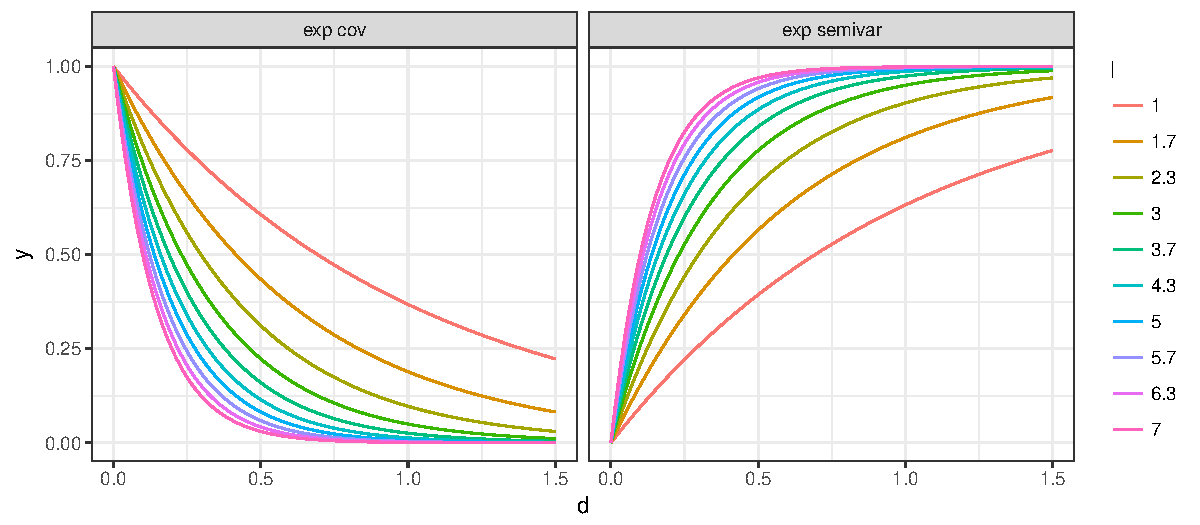
\includegraphics{Lec13_files/figure-beamer/unnamed-chunk-2-1.pdf}

\end{frame}

\begin{frame}{Covariance vs Semivariogram - Square Exponential}

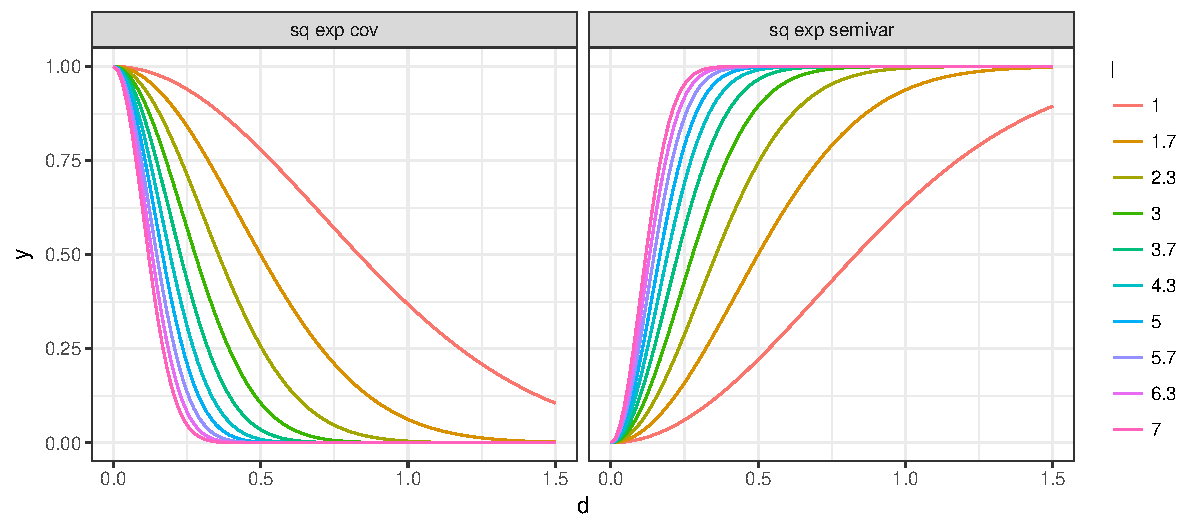
\includegraphics{Lec13_files/figure-beamer/unnamed-chunk-3-1.pdf}

\end{frame}

\begin{frame}{From last time}

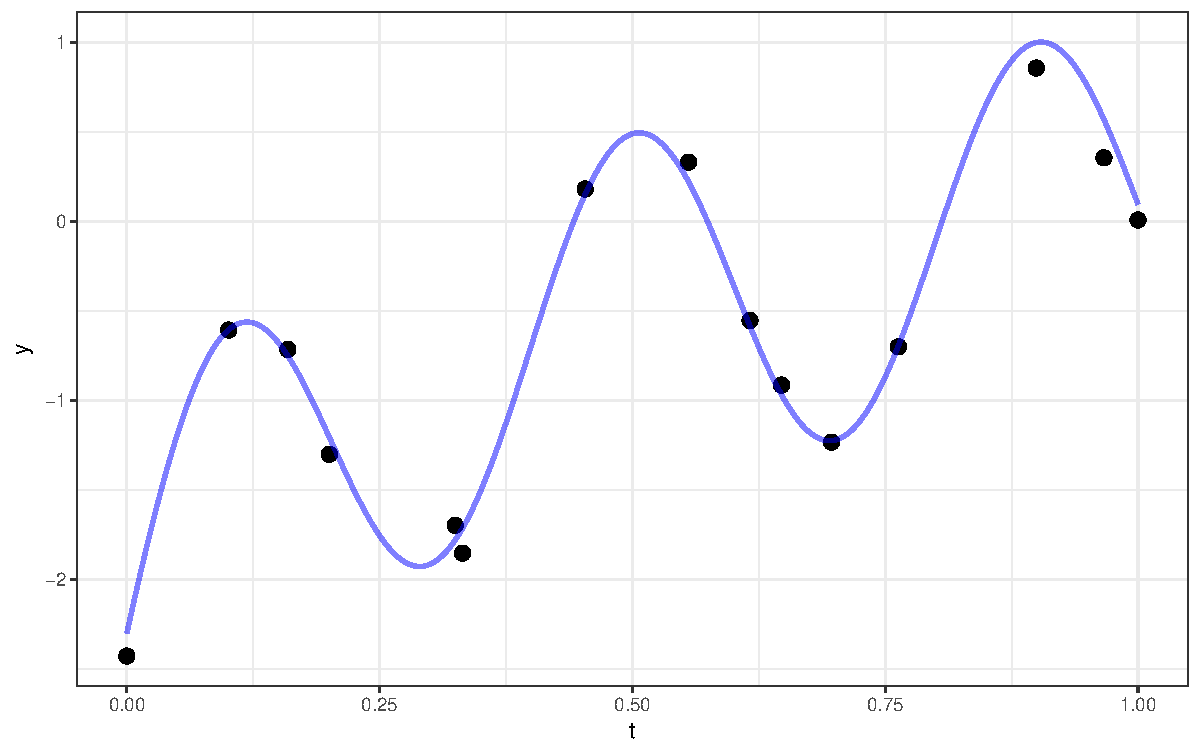
\includegraphics{Lec13_files/figure-beamer/unnamed-chunk-4-1.pdf}

\end{frame}

\begin{frame}{Empirical semivariogram - no bins / cloud}

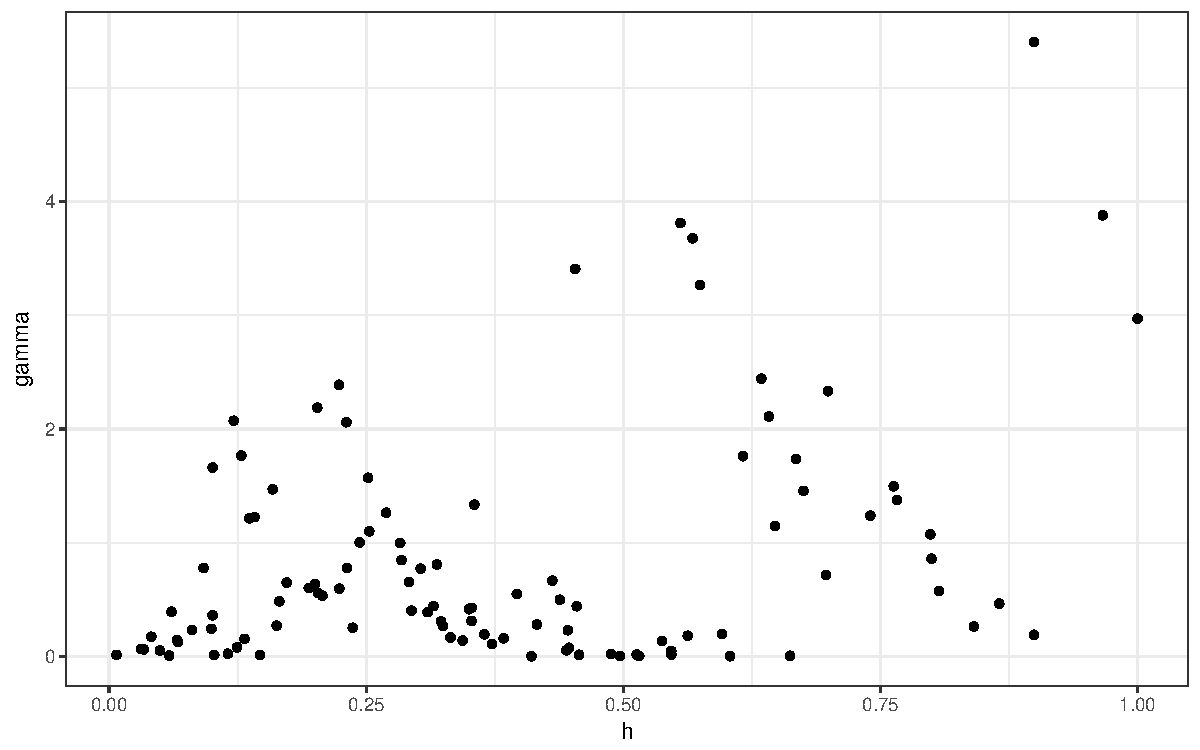
\includegraphics{Lec13_files/figure-beamer/unnamed-chunk-6-1.pdf}

\end{frame}

\begin{frame}{Empirical semivariogram (binned)}

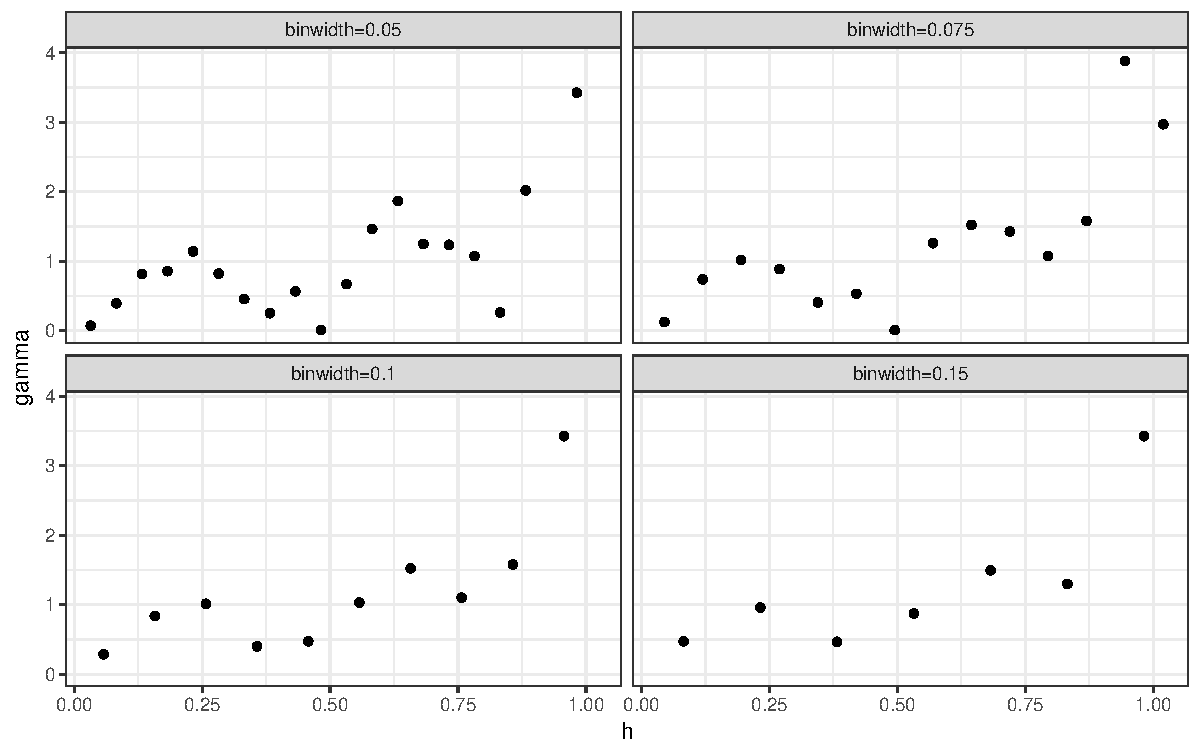
\includegraphics{Lec13_files/figure-beamer/unnamed-chunk-7-1.pdf}

\end{frame}

\begin{frame}{Empirical semivariogram (binned + n)}

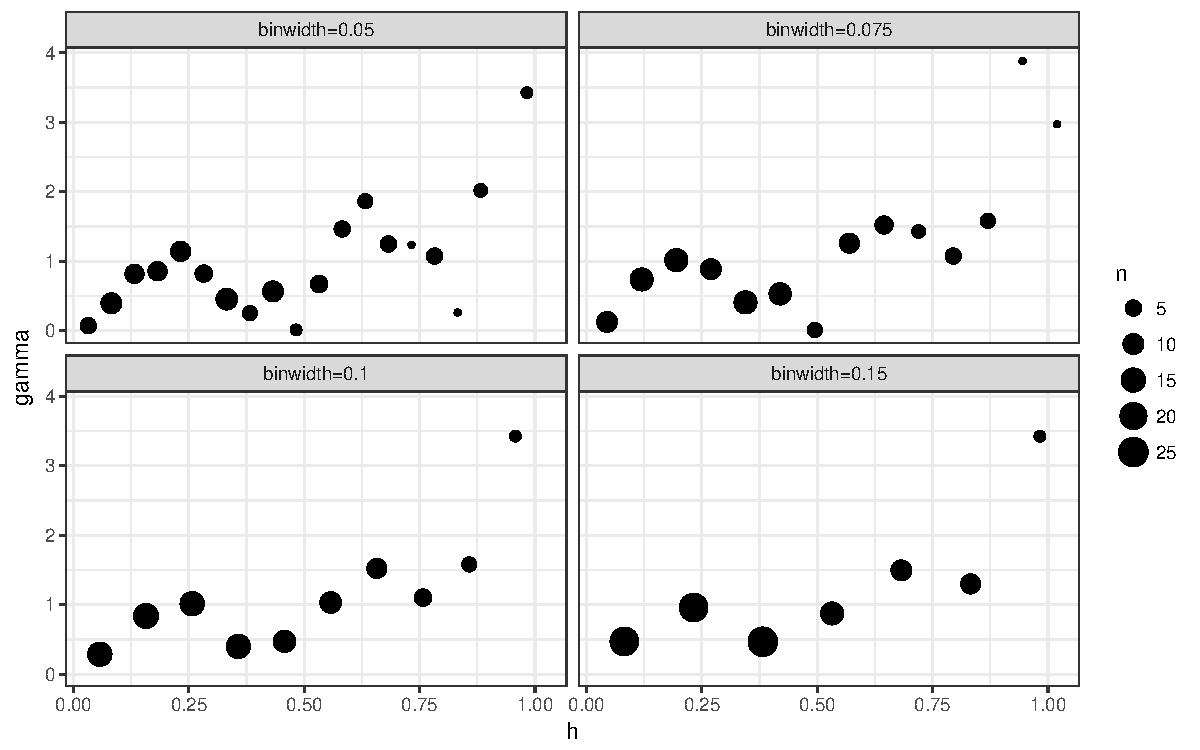
\includegraphics{Lec13_files/figure-beamer/unnamed-chunk-8-1.pdf}

\end{frame}

\begin{frame}{Theoretical vs empirical semivariogram}

After fitting the model last time we came up with a posterior median of
\(\sigma^2 = 1.89\) and \(l=5.86\) for a square exponential covariance.

\pause

\scriptsize
\[ \begin{aligned}
Cov(h) &= \sigma^2 \exp\big(-(h\,l)^2\big) \\
\gamma(h) 
  &= \sigma^2 - \sigma^2 \exp\big(-(h\,l)^2\big) \\
  &= 1.89 - 1.89 \exp\big(-(5.86\, h)^2\big)
\end{aligned}\]

\pause

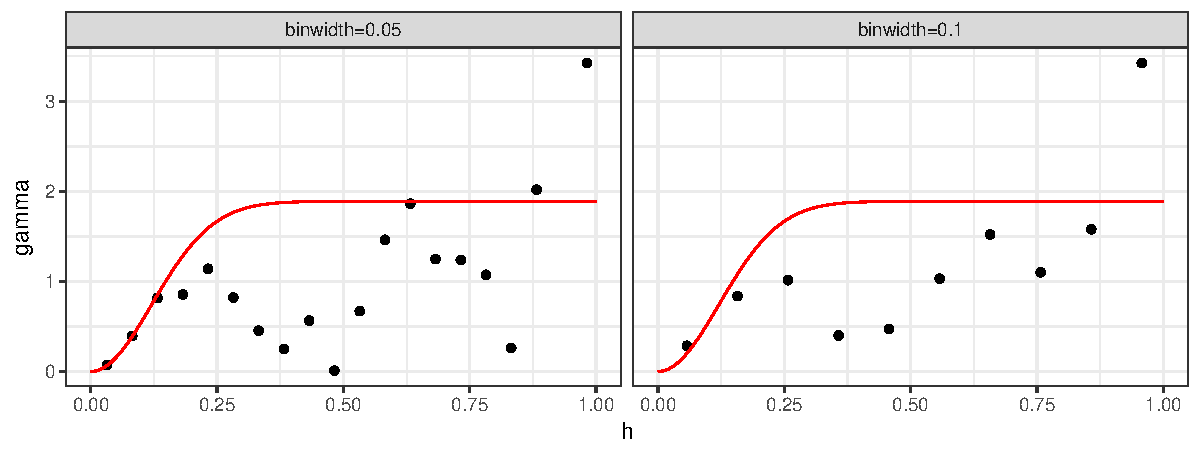
\includegraphics{Lec13_files/figure-beamer/unnamed-chunk-9-1.pdf}

\end{frame}

\begin{frame}{Variogram features}

\begin{center}
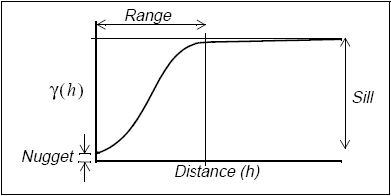
\includegraphics[width=0.7\textwidth]{figs/variogram.png}
\end{center}

\end{frame}

\section{PM2.5 Example}\label{pm2.5-example}

\begin{frame}{FRN Data}

Measured PM2.5 data from an EPA monitoring station in Columbia, NJ.

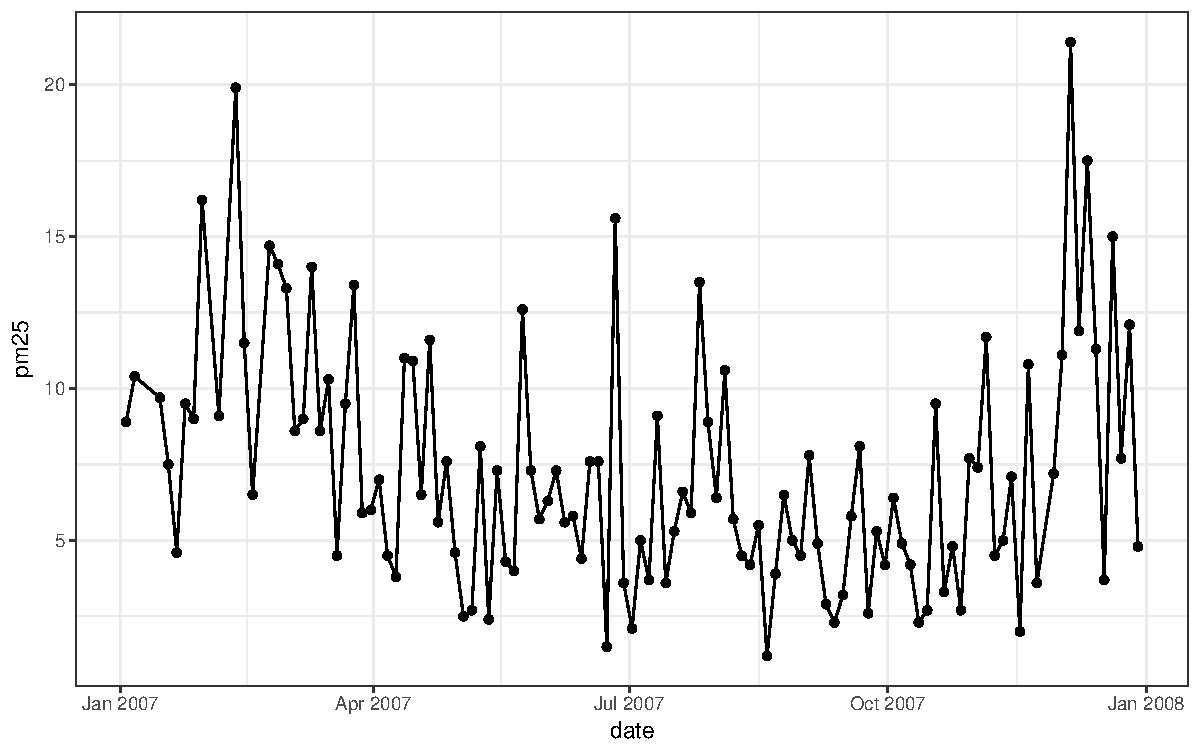
\includegraphics{Lec13_files/figure-beamer/unnamed-chunk-10-1.pdf}

\end{frame}

\begin{frame}{FRN Data}

\footnotesize

\begin{longtable}[]{@{}lrrrlr@{}}
\toprule
site & latitude & longitude & pm25 & date & day\tabularnewline
\midrule
\endhead
230031011 & 46.682 & -68.016 & 8.9 & 2007-01-03 & 3\tabularnewline
230031011 & 46.682 & -68.016 & 10.4 & 2007-01-06 & 6\tabularnewline
230031011 & 46.682 & -68.016 & 9.7 & 2007-01-15 & 15\tabularnewline
230031011 & 46.682 & -68.016 & 7.5 & 2007-01-18 & 18\tabularnewline
230031011 & 46.682 & -68.016 & 4.6 & 2007-01-21 & 21\tabularnewline
230031011 & 46.682 & -68.016 & 9.5 & 2007-01-24 & 24\tabularnewline
230031011 & 46.682 & -68.016 & 9.0 & 2007-01-27 & 27\tabularnewline
230031011 & 46.682 & -68.016 & 16.2 & 2007-01-30 & 30\tabularnewline
230031011 & 46.682 & -68.016 & 9.1 & 2007-02-05 & 36\tabularnewline
230031011 & 46.682 & -68.016 & 19.9 & 2007-02-11 & 42\tabularnewline
230031011 & 46.682 & -68.016 & 11.5 & 2007-02-14 & 45\tabularnewline
230031011 & 46.682 & -68.016 & 6.5 & 2007-02-17 & 48\tabularnewline
230031011 & 46.682 & -68.016 & 14.7 & 2007-02-23 & 54\tabularnewline
230031011 & 46.682 & -68.016 & 14.1 & 2007-02-26 & 57\tabularnewline
230031011 & 46.682 & -68.016 & 13.3 & 2007-03-01 & 60\tabularnewline
230031011 & 46.682 & -68.016 & 8.6 & 2007-03-04 & 63\tabularnewline
230031011 & 46.682 & -68.016 & 9.0 & 2007-03-07 & 66\tabularnewline
230031011 & 46.682 & -68.016 & 14.0 & 2007-03-10 & 69\tabularnewline
230031011 & 46.682 & -68.016 & 8.6 & 2007-03-13 & 72\tabularnewline
230031011 & 46.682 & -68.016 & 10.3 & 2007-03-16 & 75\tabularnewline
\bottomrule
\end{longtable}

\end{frame}

\begin{frame}[fragile]{Mean Model}

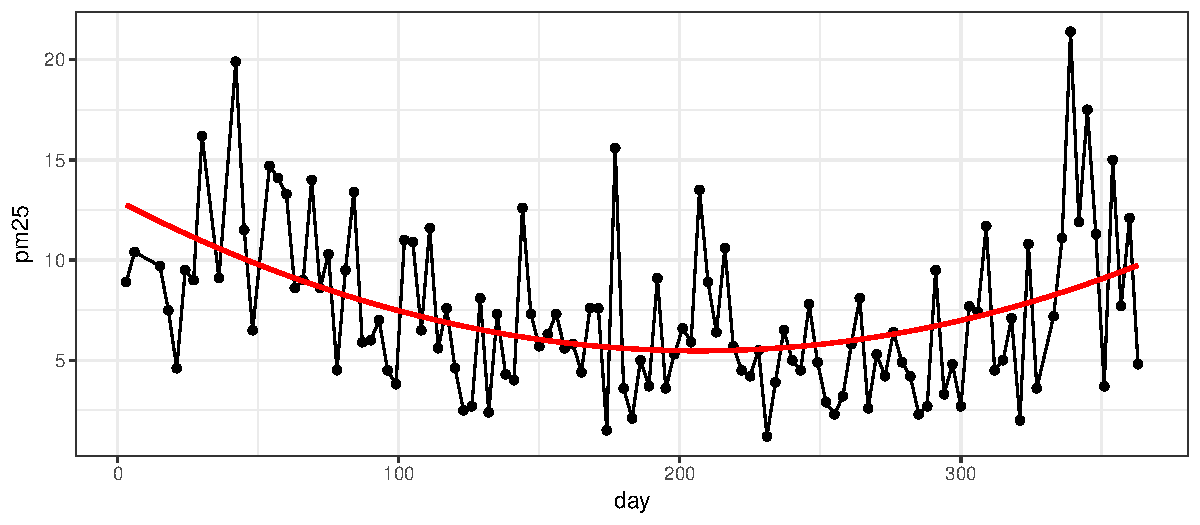
\includegraphics{Lec13_files/figure-beamer/unnamed-chunk-12-1.pdf}

\begin{verbatim}
## 
## Call:
## lm(formula = pm25 ~ day + I(day^2), data = pm25)
## 
## Coefficients:
## (Intercept)          day     I(day^2)  
##  12.9644351   -0.0724639    0.0001751
## 
## Call:
## lm(formula = pm25 ~ day + I(day^2), data = pm25)
## 
## Coefficients:
## (Intercept)          day     I(day^2)  
##  12.9644351   -0.0724639    0.0001751
\end{verbatim}

\end{frame}

\begin{frame}{Detrended Residuals}

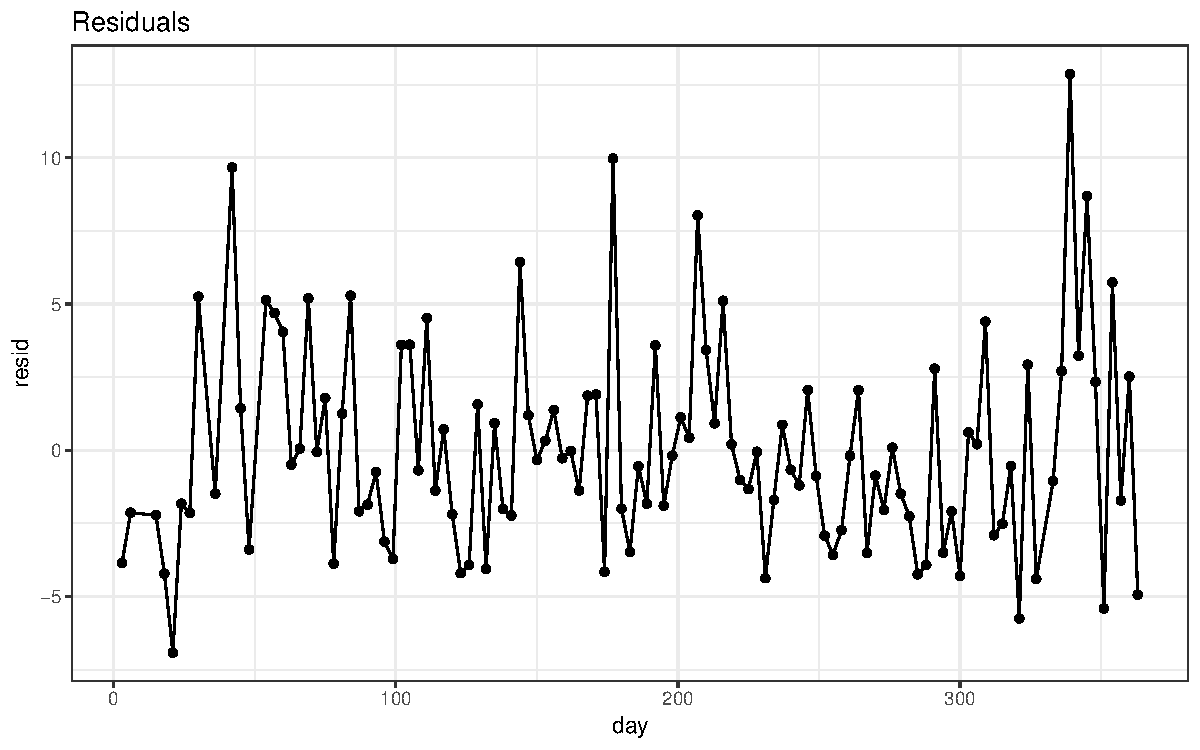
\includegraphics{Lec13_files/figure-beamer/unnamed-chunk-13-1.pdf}

\end{frame}

\begin{frame}{Empirical Variogram}

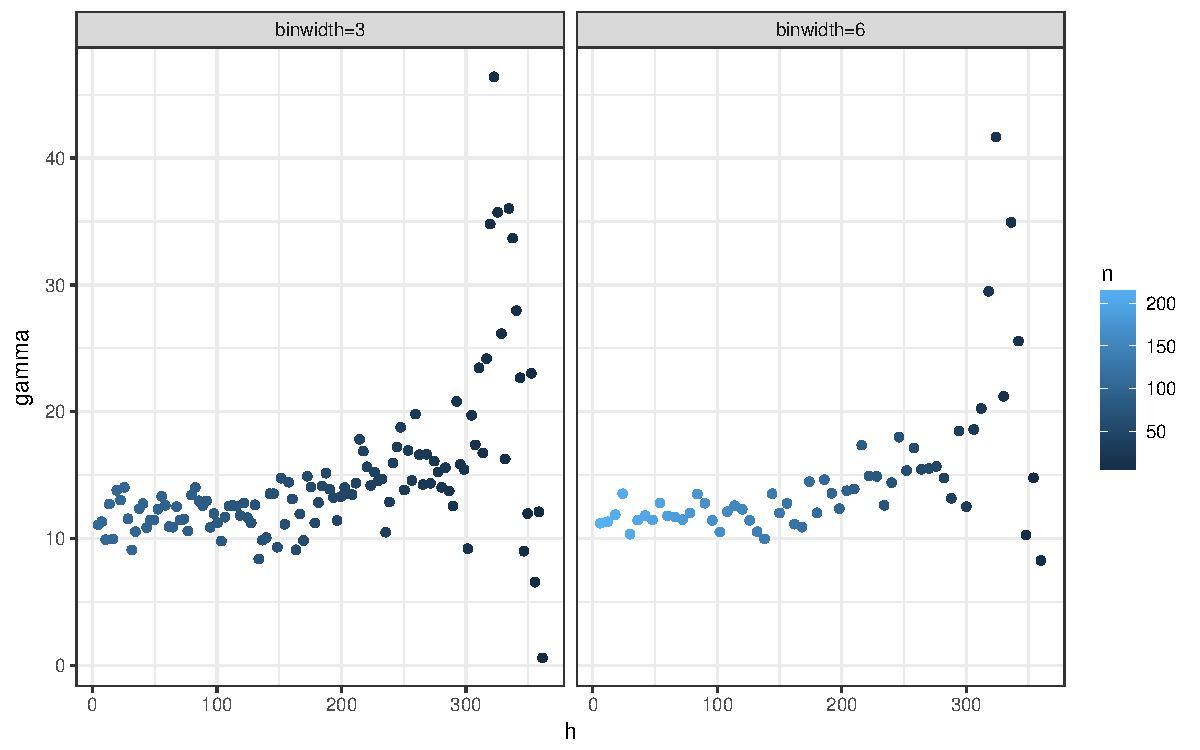
\includegraphics{Lec13_files/figure-beamer/unnamed-chunk-14-1.pdf}

\end{frame}

\begin{frame}{Empirical Variogram}

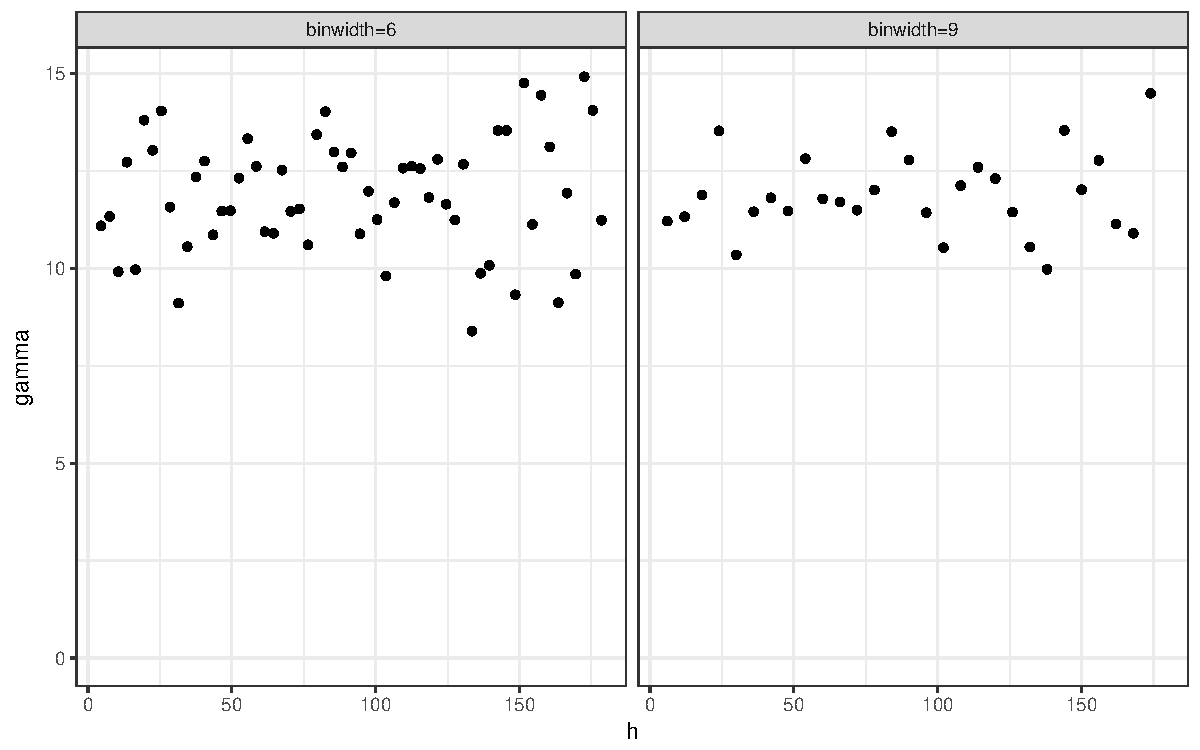
\includegraphics{Lec13_files/figure-beamer/unnamed-chunk-15-1.pdf}

\end{frame}

\begin{frame}[t]{Model}

What does the model we are trying to fit actually look like?

\pause

\vspace{2mm}

\[ y(d) = \mu(d) + w(d) + w \] where

\[\begin{aligned}
\mu(d) &= \beta0 + \beta_1\, d +\beta_2\, d^2\\
w(d) &\sim \mathcal{GP}(0, \Sigma) \\
w &\sim \mathcal{N}(0, \sigma^2_w)
\end{aligned}\]

\end{frame}

\begin{frame}[fragile]{JAGS Model}

\scriptoutput

\begin{verbatim}
## model{
##   y ~ dmnorm(mu, inverse(Sigma))
## 
##   for (i in 1:N) {
##     mu[i] <- beta[1]+ beta[2] * x[i] + beta[3] * x[i]^2
##   }
##   
##   for (i in 1:(N-1)) {
##     for (j in (i+1):N) {
##       Sigma[i,j] <- sigma2 * exp(- pow(l*d[i,j],2))
##       Sigma[j,i] <- Sigma[i,j]
##     }
##   }
## 
##   for (k in 1:N) {
##     Sigma[k,k] <- sigma2 + sigma2_w
##   }
## 
##   for (i in 1:3) {
##     beta[i] ~ dt(0, 2.5, 1)
##   }
##   sigma2_w ~ dnorm(10, 1/25) T(0,)
##   sigma2   ~ dnorm(10, 1/25) T(0,)
##   l        ~ dt(0, 2.5, 1) T(0,) 
## }
\end{verbatim}

\end{frame}

\begin{frame}{Posterior - Betas}

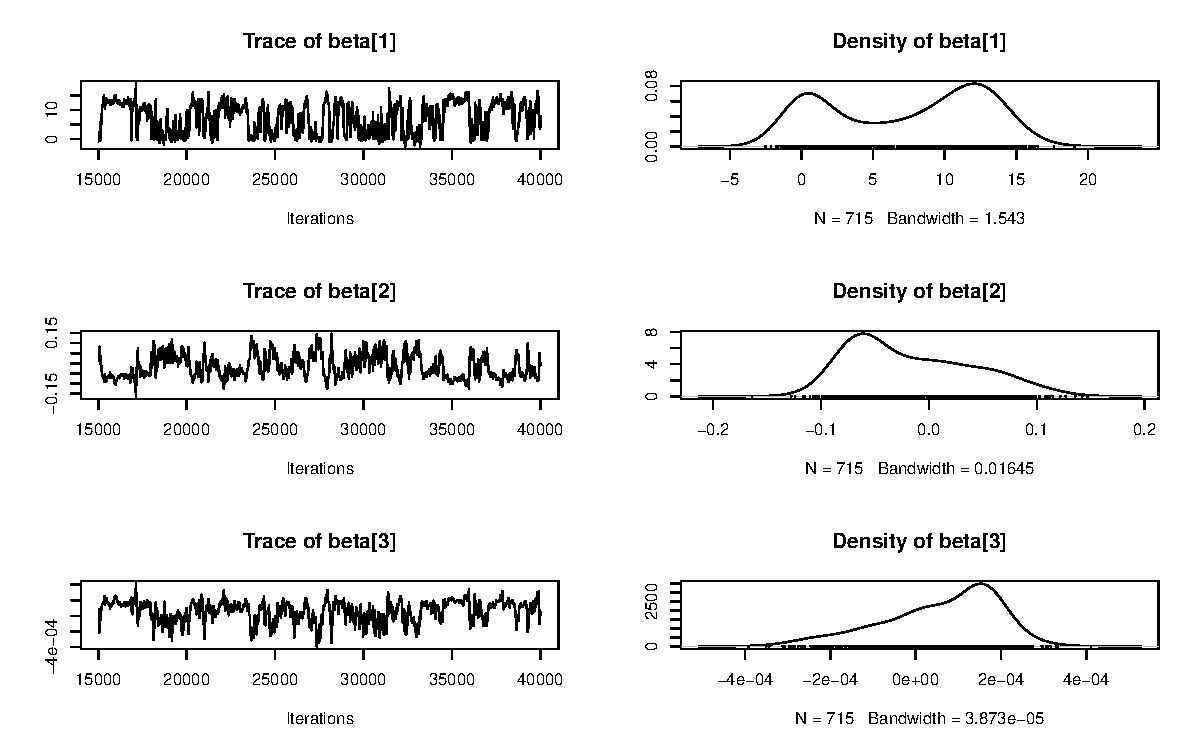
\includegraphics{Lec13_files/figure-beamer/unnamed-chunk-18-1.pdf}

\end{frame}

\begin{frame}{Posterior - Covariance Parameters}

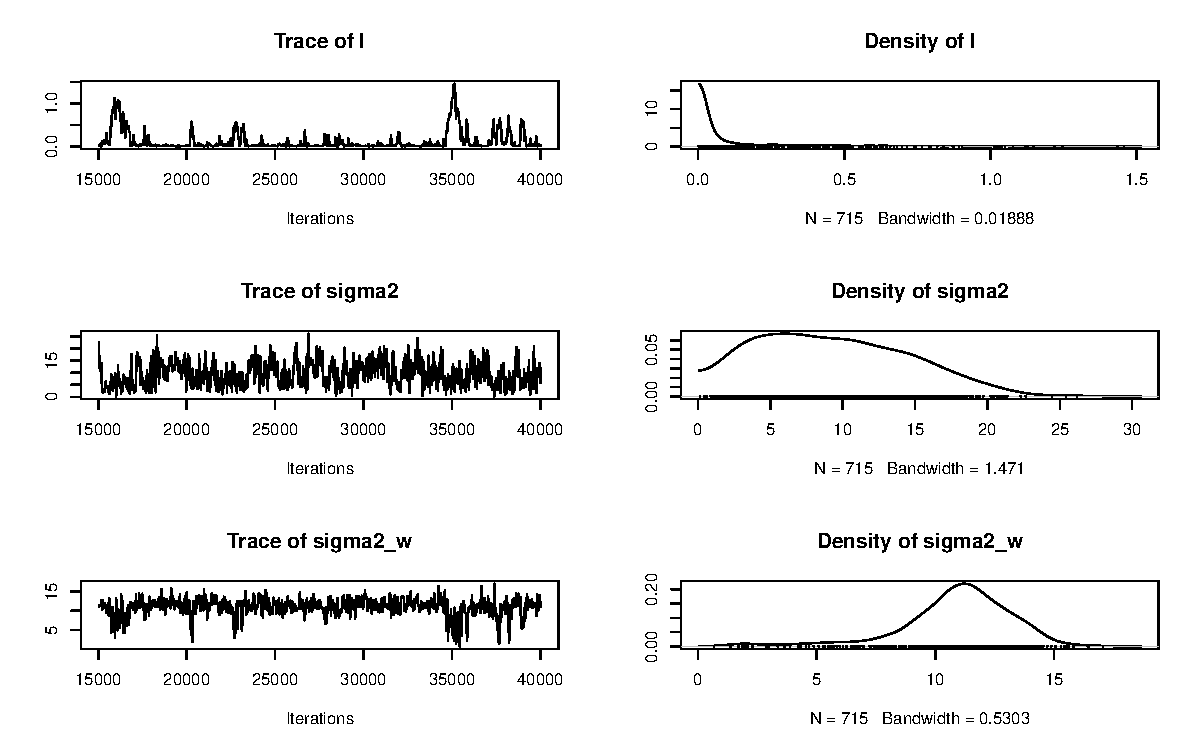
\includegraphics{Lec13_files/figure-beamer/unnamed-chunk-19-1.pdf}

\end{frame}

\begin{frame}[fragile]{Posterior}

\begin{verbatim}
## # A tibble: 6 × 5
##      param     post_mean      post_med    post_lower   post_upper
## *    <chr>         <dbl>         <dbl>         <dbl>        <dbl>
## 1  beta[1]  7.283488e+00  8.667009e+00 -0.7461648059 1.503065e+01
## 2  beta[2] -1.627421e-02 -2.817415e-02 -0.0988863015 1.026401e-01
## 3  beta[3]  5.858818e-05  8.569993e-05 -0.0002481874 2.567976e-04
## 4        l  1.277712e-01  2.433287e-02  0.0060909947 8.443888e-01
## 5   sigma2  9.379213e+00  9.016621e+00  1.5643832453 1.979094e+01
## 6 sigma2_w  1.088809e+01  1.116626e+01  4.2665826402 1.448447e+01
\end{verbatim}

\end{frame}

\begin{frame}{Fitted Variogram}

\end{frame}

\begin{frame}{Empirical + Fitted Variogram}

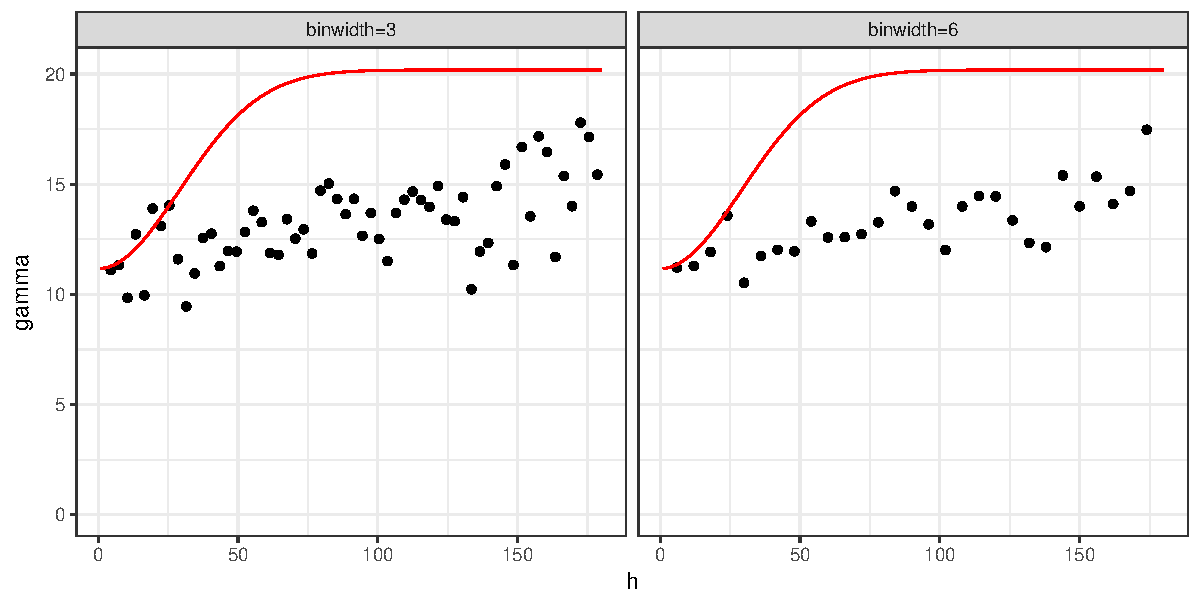
\includegraphics{Lec13_files/figure-beamer/unnamed-chunk-21-1.pdf}

\end{frame}

\begin{frame}{Fitted Model + Predictions}

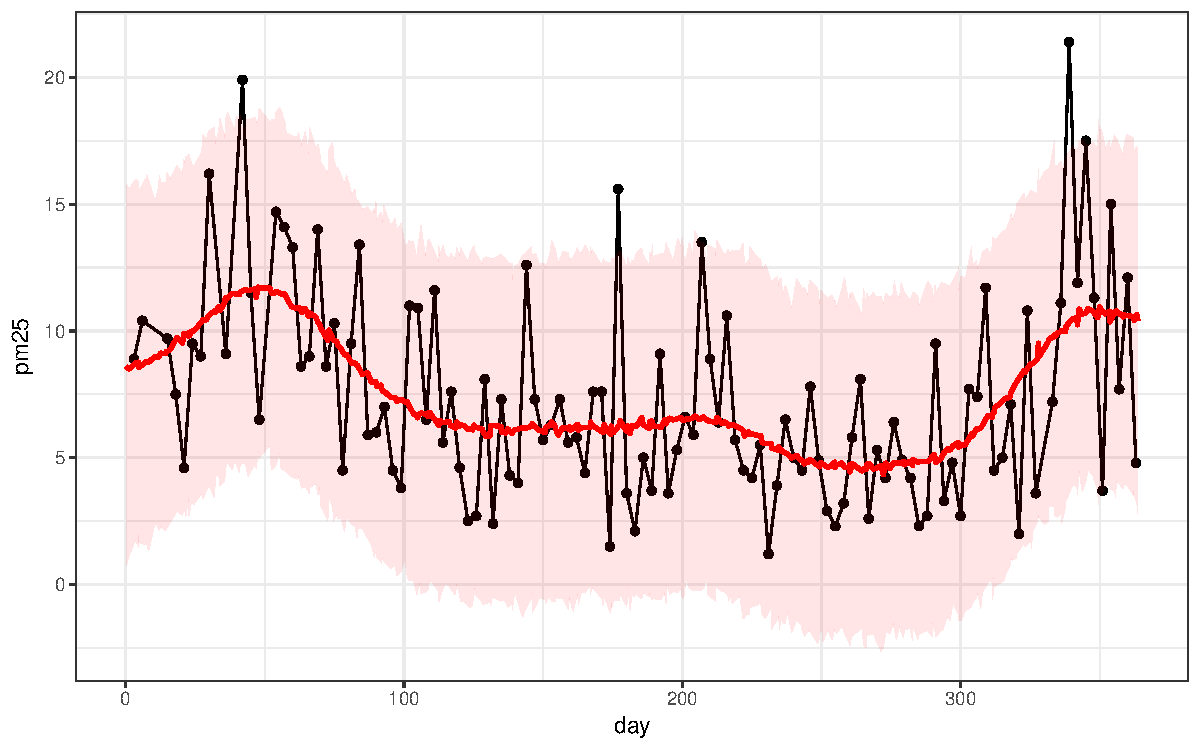
\includegraphics{Lec13_files/figure-beamer/unnamed-chunk-22-1.pdf}

\end{frame}

\begin{frame}{Empirical Variogram (again)}

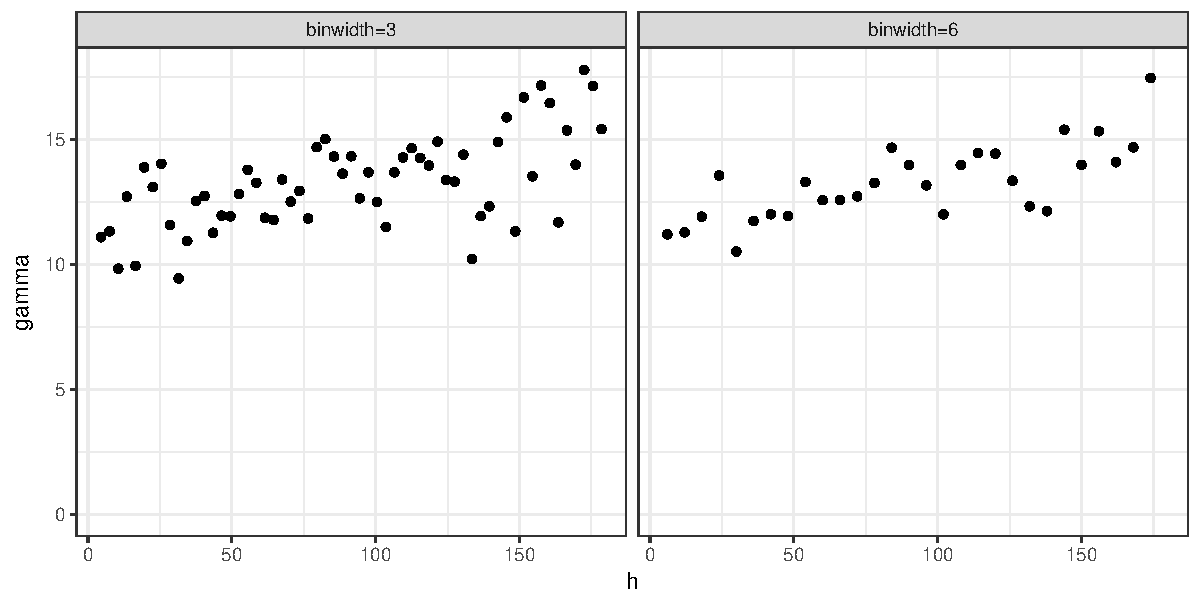
\includegraphics{Lec13_files/figure-beamer/unnamed-chunk-23-1.pdf}

\end{frame}

\begin{frame}{Empirical Variogram Model}

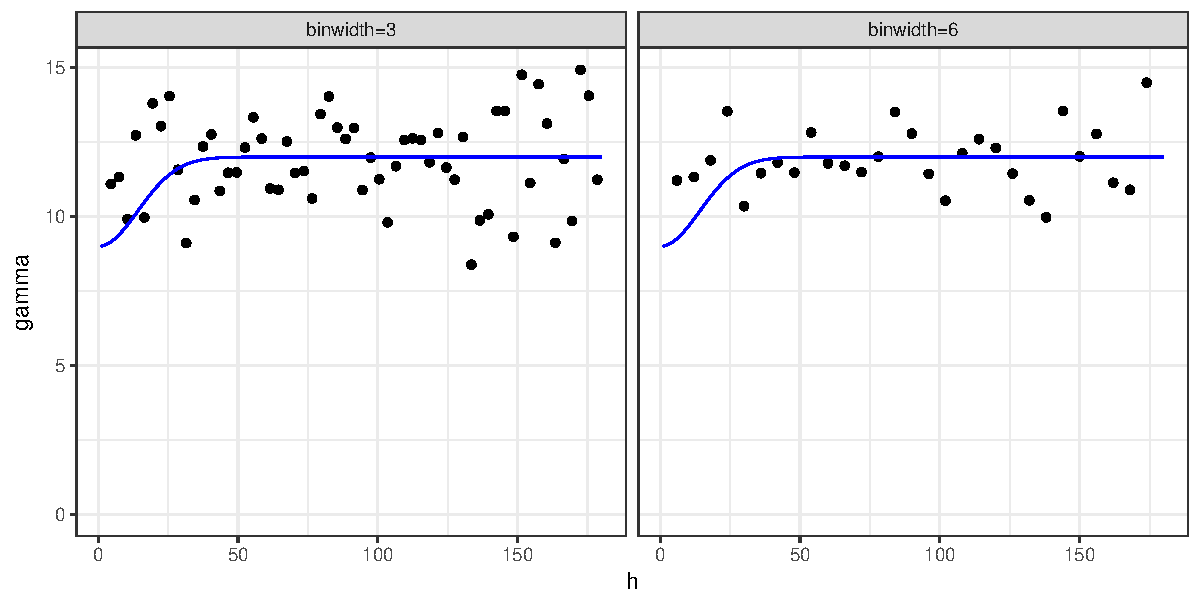
\includegraphics{Lec13_files/figure-beamer/unnamed-chunk-24-1.pdf}

\end{frame}

\begin{frame}{Empirical Variogram Model + Predictions}

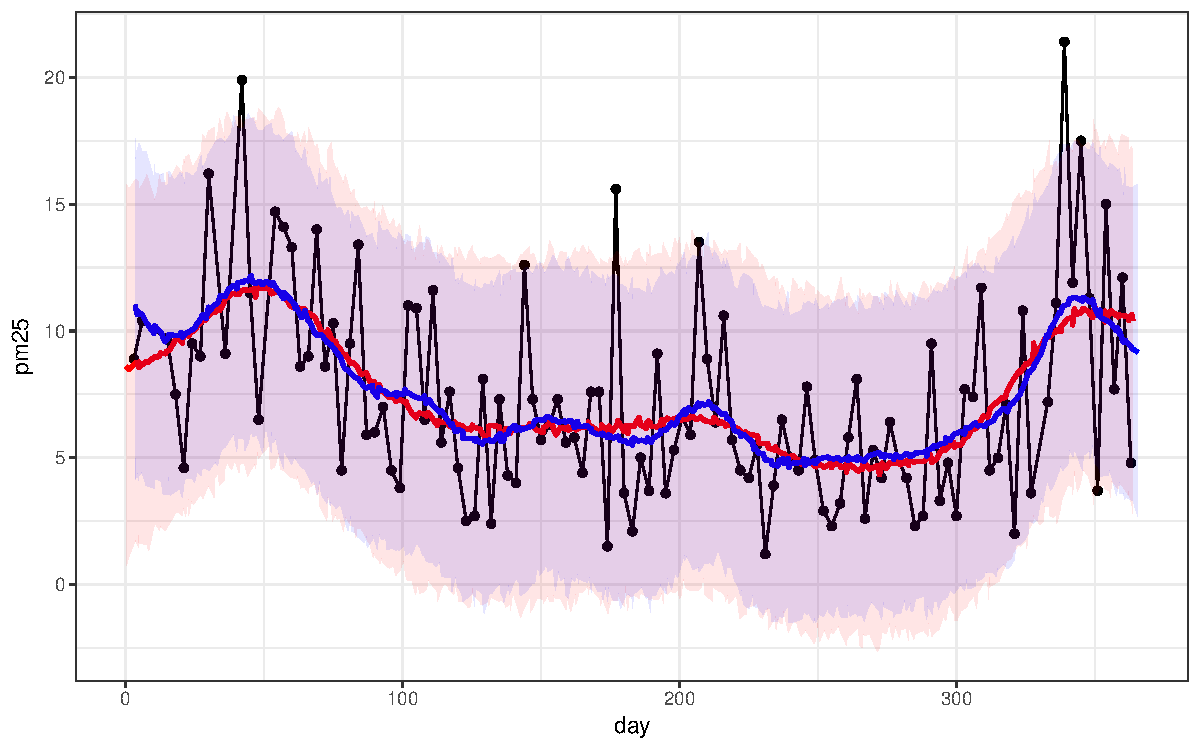
\includegraphics{Lec13_files/figure-beamer/unnamed-chunk-25-1.pdf}

\end{frame}

\end{document}
